\documentclass[1p]{elsarticle_modified}
%\bibliographystyle{elsarticle-num}

%\usepackage[colorlinks]{hyperref}
%\usepackage{abbrmath_seonhwa} %\Abb, \Ascr, \Acal ,\Abf, \Afrak
\usepackage{amsfonts}
\usepackage{amssymb}
\usepackage{amsmath}
\usepackage{amsthm}
\usepackage{scalefnt}
\usepackage{amsbsy}
\usepackage{kotex}
\usepackage{caption}
\usepackage{subfig}
\usepackage{color}
\usepackage{graphicx}
\usepackage{xcolor} %% white, black, red, green, blue, cyan, magenta, yellow
\usepackage{float}
\usepackage{setspace}
\usepackage{hyperref}

\usepackage{tikz}
\usetikzlibrary{arrows}

\usepackage{multirow}
\usepackage{array} % fixed length table
\usepackage{hhline}

%%%%%%%%%%%%%%%%%%%%%
\makeatletter
\renewcommand*\env@matrix[1][\arraystretch]{%
	\edef\arraystretch{#1}%
	\hskip -\arraycolsep
	\let\@ifnextchar\new@ifnextchar
	\array{*\c@MaxMatrixCols c}}
\makeatother %https://tex.stackexchange.com/questions/14071/how-can-i-increase-the-line-spacing-in-a-matrix
%%%%%%%%%%%%%%%

\usepackage[normalem]{ulem}

\newcommand{\msout}[1]{\ifmmode\text{\sout{\ensuremath{#1}}}\else\sout{#1}\fi}
%SOURCE: \msout is \stkout macro in https://tex.stackexchange.com/questions/20609/strikeout-in-math-mode

\newcommand{\cancel}[1]{
	\ifmmode
	{\color{red}\msout{#1}}
	\else
	{\color{red}\sout{#1}}
	\fi
}

\newcommand{\add}[1]{
	{\color{blue}\uwave{#1}}
}

\newcommand{\replace}[2]{
	\ifmmode
	{\color{red}\msout{#1}}{\color{blue}\uwave{#2}}
	\else
	{\color{red}\sout{#1}}{\color{blue}\uwave{#2}}
	\fi
}

\newcommand{\Sol}{\mathcal{S}} %segment
\newcommand{\D}{D} %diagram
\newcommand{\A}{\mathcal{A}} %arc


%%%%%%%%%%%%%%%%%%%%%%%%%%%%%5 test

\def\sl{\operatorname{\textup{SL}}(2,\Cbb)}
\def\psl{\operatorname{\textup{PSL}}(2,\Cbb)}
\def\quan{\mkern 1mu \triangleright \mkern 1mu}

\theoremstyle{definition}
\newtheorem{thm}{Theorem}[section]
\newtheorem{prop}[thm]{Proposition}
\newtheorem{lem}[thm]{Lemma}
\newtheorem{ques}[thm]{Question}
\newtheorem{cor}[thm]{Corollary}
\newtheorem{defn}[thm]{Definition}
\newtheorem{exam}[thm]{Example}
\newtheorem{rmk}[thm]{Remark}
\newtheorem{alg}[thm]{Algorithm}

\newcommand{\I}{\sqrt{-1}}
\begin{document}

%\begin{frontmatter}
%
%\title{Boundary parabolic representations of knots up to 8 crossings}
%
%%% Group authors per affiliation:
%\author{Yunhi Cho} 
%\address{Department of Mathematics, University of Seoul, Seoul, Korea}
%\ead{yhcho@uos.ac.kr}
%
%
%\author{Seonhwa Kim} %\fnref{s_kim}}
%\address{Center for Geometry and Physics, Institute for Basic Science, Pohang, 37673, Korea}
%\ead{ryeona17@ibs.re.kr}
%
%\author{Hyuk Kim}
%\address{Department of Mathematical Sciences, Seoul National University, Seoul 08826, Korea}
%\ead{hyukkim@snu.ac.kr}
%
%\author{Seokbeom Yoon}
%\address{Department of Mathematical Sciences, Seoul National University, Seoul, 08826,  Korea}
%\ead{sbyoon15@snu.ac.kr}
%
%\begin{abstract}
%We find all boundary parabolic representation of knots up to 8 crossings.
%
%\end{abstract}
%\begin{keyword}
%    \MSC[2010] 57M25 
%\end{keyword}
%
%\end{frontmatter}

%\linenumbers
%\tableofcontents
%
\newcommand\colored[1]{\textcolor{white}{\rule[-0.35ex]{0.8em}{1.4ex}}\kern-0.8em\color{red} #1}%
%\newcommand\colored[1]{\textcolor{white}{ #1}\kern-2.17ex	\textcolor{white}{ #1}\kern-1.81ex	\textcolor{white}{ #1}\kern-2.15ex\color{red}#1	}

{\Large $\underline{11a_{273}~(K11a_{273})}$}

\setlength{\tabcolsep}{10pt}
\renewcommand{\arraystretch}{1.6}
\vspace{1cm}\begin{tabular}{m{100pt}>{\centering\arraybackslash}m{274pt}}
\multirow{5}{120pt}{
	\centering
	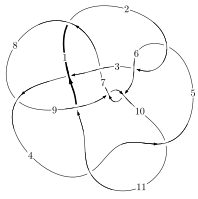
\includegraphics[width=112pt]{../../../GIT/diagram.site/Diagrams/png/522_11a_273.png}\\
\ \ \ A knot diagram\footnotemark}&
\allowdisplaybreaks
\textbf{Linearized knot diagam} \\
\cline{2-2}
 &
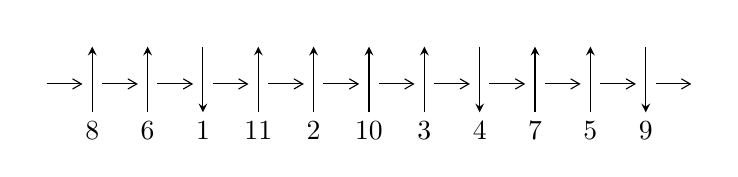
\begin{tikzpicture}[x=20pt, y=17pt]
	% nodes
	\node (C0) at (0, 0) {};
	\node (C1) at (1, 0) {};
	\node (C1U) at (1, +1) {};
	\node (C1D) at (1, -1) {8};

	\node (C2) at (2, 0) {};
	\node (C2U) at (2, +1) {};
	\node (C2D) at (2, -1) {6};

	\node (C3) at (3, 0) {};
	\node (C3U) at (3, +1) {};
	\node (C3D) at (3, -1) {1};

	\node (C4) at (4, 0) {};
	\node (C4U) at (4, +1) {};
	\node (C4D) at (4, -1) {11};

	\node (C5) at (5, 0) {};
	\node (C5U) at (5, +1) {};
	\node (C5D) at (5, -1) {2};

	\node (C6) at (6, 0) {};
	\node (C6U) at (6, +1) {};
	\node (C6D) at (6, -1) {10};

	\node (C7) at (7, 0) {};
	\node (C7U) at (7, +1) {};
	\node (C7D) at (7, -1) {3};

	\node (C8) at (8, 0) {};
	\node (C8U) at (8, +1) {};
	\node (C8D) at (8, -1) {4};

	\node (C9) at (9, 0) {};
	\node (C9U) at (9, +1) {};
	\node (C9D) at (9, -1) {7};

	\node (C10) at (10, 0) {};
	\node (C10U) at (10, +1) {};
	\node (C10D) at (10, -1) {5};

	\node (C11) at (11, 0) {};
	\node (C11U) at (11, +1) {};
	\node (C11D) at (11, -1) {9};
	\node (C12) at (12, 0) {};

	% arrows
	\draw[->,>={angle 60}]
	(C0) edge (C1) (C1) edge (C2) (C2) edge (C3) (C3) edge (C4) (C4) edge (C5) (C5) edge (C6) (C6) edge (C7) (C7) edge (C8) (C8) edge (C9) (C9) edge (C10) (C10) edge (C11) (C11) edge (C12) ;	\draw[->,>=stealth]
	(C1D) edge (C1U) (C2D) edge (C2U) (C3U) edge (C3D) (C4D) edge (C4U) (C5D) edge (C5U) (C6D) edge (C6U) (C7D) edge (C7U) (C8U) edge (C8D) (C9D) edge (C9U) (C10D) edge (C10U) (C11U) edge (C11D) ;
	\end{tikzpicture} \\
\hhline{~~} \\& 
\textbf{Solving Sequence} \\ \cline{2-2} 
 &
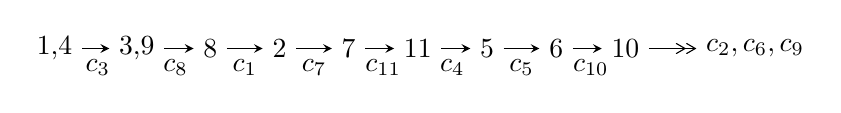
\begin{tikzpicture}[x=25pt, y=7pt]
	% node
	\node (A0) at (-1/8, 0) {1,4};
	\node (A1) at (17/16, 0) {3,9};
	\node (A2) at (17/8, 0) {8};
	\node (A3) at (25/8, 0) {2};
	\node (A4) at (33/8, 0) {7};
	\node (A5) at (41/8, 0) {11};
	\node (A6) at (49/8, 0) {5};
	\node (A7) at (57/8, 0) {6};
	\node (A8) at (65/8, 0) {10};
	\node (C1) at (1/2, -1) {$c_{3}$};
	\node (C2) at (13/8, -1) {$c_{8}$};
	\node (C3) at (21/8, -1) {$c_{1}$};
	\node (C4) at (29/8, -1) {$c_{7}$};
	\node (C5) at (37/8, -1) {$c_{11}$};
	\node (C6) at (45/8, -1) {$c_{4}$};
	\node (C7) at (53/8, -1) {$c_{5}$};
	\node (C8) at (61/8, -1) {$c_{10}$};
	\node (A9) at (10, 0) {$c_{2},c_{6},c_{9}$};

	% edge
	\draw[->,>=stealth]	
	(A0) edge (A1) (A1) edge (A2) (A2) edge (A3) (A3) edge (A4) (A4) edge (A5) (A5) edge (A6) (A6) edge (A7) (A7) edge (A8) ;
	\draw[->>,>={angle 60}]	
	(A8) edge (A9);
\end{tikzpicture} \\ 

\end{tabular} \\

\footnotetext{
The image of knot diagram is generated by the software ``\textbf{Draw programme}" developed by Andrew Bartholomew(\url{http://www.layer8.co.uk/maths/draw/index.htm\#Running-draw}), where we modified some parts for our purpose(\url{https://github.com/CATsTAILs/LinksPainter}).
}\phantom \\ \newline 
\centering \textbf{Ideals for irreducible components\footnotemark of $X_{\text{par}}$} 
 
\begin{align*}
I^u_{1}&=\langle 
1.06666\times10^{485} u^{100}-3.41235\times10^{486} u^{99}+\cdots+2.42206\times10^{486} b+4.73084\times10^{487},\\
\phantom{I^u_{1}}&\phantom{= \langle  }-3.39554\times10^{486} u^{100}+9.74479\times10^{486} u^{99}+\cdots+2.42206\times10^{486} a-6.95932\times10^{487},\\
\phantom{I^u_{1}}&\phantom{= \langle  }2 u^{101}-3 u^{100}+\cdots+35 u-7\rangle \\
I^u_{2}&=\langle 
61808523107 u^{19}+536394633246 u^{18}+\cdots+299510947709 b+100240238594,\\
\phantom{I^u_{2}}&\phantom{= \langle  }68387457437 u^{19}+547043741023 u^{18}+\cdots+299510947709 a+331101363754,\\
\phantom{I^u_{2}}&\phantom{= \langle  }u^{20}+8 u^{19}+\cdots+2 u^2+1\rangle \\
I^u_{3}&=\langle 
b-2 u+1,\;a,\;2 u^2- u+1\rangle \\
\\
\end{align*}
\raggedright * 3 irreducible components of $\dim_{\mathbb{C}}=0$, with total 123 representations.\\
\footnotetext{All coefficients of polynomials are rational numbers. But the coefficients are sometimes approximated in decimal forms when there is not enough margin.}
\newpage
\renewcommand{\arraystretch}{1}
\centering \section*{I. $I^u_{1}= \langle 1.07\times10^{485} u^{100}-3.41\times10^{486} u^{99}+\cdots+2.42\times10^{486} b+4.73\times10^{487},\;-3.40\times10^{486} u^{100}+9.74\times10^{486} u^{99}+\cdots+2.42\times10^{486} a-6.96\times10^{487},\;2 u^{101}-3 u^{100}+\cdots+35 u-7 \rangle$}
\flushleft \textbf{(i) Arc colorings}\\
\begin{tabular}{m{7pt} m{180pt} m{7pt} m{180pt} }
\flushright $a_{1}=$&$\begin{pmatrix}0\\u\end{pmatrix}$ \\
\flushright $a_{4}=$&$\begin{pmatrix}1\\0\end{pmatrix}$ \\
\flushright $a_{3}=$&$\begin{pmatrix}1\\- u^2\end{pmatrix}$ \\
\flushright $a_{9}=$&$\begin{pmatrix}1.40192 u^{100}-4.02334 u^{99}+\cdots-94.7128 u+28.7330\\-0.0440391 u^{100}+1.40886 u^{99}+\cdots+98.4076 u-19.5323\end{pmatrix}$ \\
\flushright $a_{8}=$&$\begin{pmatrix}1.35788 u^{100}-2.61448 u^{99}+\cdots+3.69486 u+9.20073\\-0.0440391 u^{100}+1.40886 u^{99}+\cdots+98.4076 u-19.5323\end{pmatrix}$ \\
\flushright $a_{2}=$&$\begin{pmatrix}5.77692 u^{100}-6.87002 u^{99}+\cdots-77.9350 u+9.89514\\1.01775 u^{100}-0.0986016 u^{99}+\cdots+65.2026 u-18.2878\end{pmatrix}$ \\
\flushright $a_{7}=$&$\begin{pmatrix}3.21671 u^{100}-5.97036 u^{99}+\cdots-109.574 u+30.7548\\0.231287 u^{100}+0.930191 u^{99}+\cdots+81.9680 u-17.5456\end{pmatrix}$ \\
\flushright $a_{11}=$&$\begin{pmatrix}6.07414 u^{100}-8.70607 u^{99}+\cdots-188.680 u+36.7620\\-1.31496 u^{100}+1.93465 u^{99}+\cdots+47.5422 u-8.57902\end{pmatrix}$ \\
\flushright $a_{5}=$&$\begin{pmatrix}0.431473 u^{100}-4.89396 u^{99}+\cdots-178.199 u+67.0158\\-0.485513 u^{100}+0.496210 u^{99}+\cdots+3.24494 u-3.96348\end{pmatrix}$ \\
\flushright $a_{6}=$&$\begin{pmatrix}-2.82245 u^{100}+0.822439 u^{99}+\cdots-125.329 u+46.6321\\-1.90585 u^{100}+1.04687 u^{99}+\cdots-48.8140 u+12.4729\end{pmatrix}$ \\
\flushright $a_{10}=$&$\begin{pmatrix}-6.76378 u^{100}+5.57659 u^{99}+\cdots+53.5301 u+1.49940\\-1.05903 u^{100}+1.81446 u^{99}+\cdots+31.6066 u-3.21755\end{pmatrix}$\\ \flushright $a_{10}=$&$\begin{pmatrix}-6.76378 u^{100}+5.57659 u^{99}+\cdots+53.5301 u+1.49940\\-1.05903 u^{100}+1.81446 u^{99}+\cdots+31.6066 u-3.21755\end{pmatrix}$\\&\end{tabular}
\flushleft \textbf{(ii) Obstruction class $= -1$}\\~\\
\flushleft \textbf{(iii) Cusp Shapes $= -8.98950 u^{100}+8.39126 u^{99}+\cdots+221.775 u+20.5080$}\\~\\
\newpage\renewcommand{\arraystretch}{1}
\flushleft \textbf{(iv) u-Polynomials at the component}\newline \\
\begin{tabular}{m{50pt}|m{274pt}}
Crossings & \hspace{64pt}u-Polynomials at each crossing \\
\hline $$\begin{aligned}c_{1}\end{aligned}$$&$\begin{aligned}
&u^{101}-3 u^{100}+\cdots+4162 u+679
\end{aligned}$\\
\hline $$\begin{aligned}c_{2},c_{5}\end{aligned}$$&$\begin{aligned}
&u^{101}+u^{100}+\cdots-8 u-21
\end{aligned}$\\
\hline $$\begin{aligned}c_{3}\end{aligned}$$&$\begin{aligned}
&2(2 u^{101}-3 u^{100}+\cdots+35 u-7)
\end{aligned}$\\
\hline $$\begin{aligned}c_{4},c_{10}\end{aligned}$$&$\begin{aligned}
&2(2 u^{101}+5 u^{100}+\cdots-157973 u-15557)
\end{aligned}$\\
\hline $$\begin{aligned}c_{6},c_{9}\end{aligned}$$&$\begin{aligned}
&u^{101}-5 u^{100}+\cdots+2016 u+189
\end{aligned}$\\
\hline $$\begin{aligned}c_{7}\end{aligned}$$&$\begin{aligned}
&2(2 u^{101}- u^{100}+\cdots-16872 u-3626)
\end{aligned}$\\
\hline $$\begin{aligned}c_{8}\end{aligned}$$&$\begin{aligned}
&u^{101}-2 u^{100}+\cdots+4109 u-922
\end{aligned}$\\
\hline $$\begin{aligned}c_{11}\end{aligned}$$&$\begin{aligned}
&u^{101}-7 u^{100}+\cdots+278 u-48
\end{aligned}$\\
\hline
\end{tabular}\\~\\
\newpage\renewcommand{\arraystretch}{1}
\flushleft \textbf{(v) Riley Polynomials at the component}\newline \\
\begin{tabular}{m{50pt}|m{274pt}}
Crossings & \hspace{64pt}Riley Polynomials at each crossing \\
\hline $$\begin{aligned}c_{1}\end{aligned}$$&$\begin{aligned}
&y^{101}-3 y^{100}+\cdots-13847930 y-461041
\end{aligned}$\\
\hline $$\begin{aligned}c_{2},c_{5}\end{aligned}$$&$\begin{aligned}
&y^{101}-47 y^{100}+\cdots+6868 y-441
\end{aligned}$\\
\hline $$\begin{aligned}c_{3}\end{aligned}$$&$\begin{aligned}
&4(4 y^{101}-25 y^{100}+\cdots-1127 y-49)
\end{aligned}$\\
\hline $$\begin{aligned}c_{4},c_{10}\end{aligned}$$&$\begin{aligned}
&4(4 y^{101}+263 y^{100}+\cdots-2.53465\times10^{9} y-2.42020\times10^{8})
\end{aligned}$\\
\hline $$\begin{aligned}c_{6},c_{9}\end{aligned}$$&$\begin{aligned}
&y^{101}+57 y^{100}+\cdots+1976562 y-35721
\end{aligned}$\\
\hline $$\begin{aligned}c_{7}\end{aligned}$$&$\begin{aligned}
&4(4 y^{101}+11 y^{100}+\cdots+6.41717\times10^{8} y-1.31479\times10^{7})
\end{aligned}$\\
\hline $$\begin{aligned}c_{8}\end{aligned}$$&$\begin{aligned}
&y^{101}-18 y^{100}+\cdots+29207333 y-850084
\end{aligned}$\\
\hline $$\begin{aligned}c_{11}\end{aligned}$$&$\begin{aligned}
&y^{101}-27 y^{100}+\cdots+20068 y-2304
\end{aligned}$\\
\hline
\end{tabular}\\~\\
\newpage\flushleft \textbf{(vi) Complex Volumes and Cusp Shapes}
$$\begin{array}{c|c|c}  
\text{Solutions to }I^u_{1}& \I (\text{vol} + \sqrt{-1}CS) & \text{Cusp shape}\\
 \hline 
\begin{aligned}
u &= -0.162573 + 0.974272 I \\
a &= -1.262170 + 0.010151 I \\
b &= \phantom{-}1.58037 - 0.37347 I\end{aligned}
 & -0.02059 + 5.96503 I & \phantom{-0.000000 } 0 \\ \hline\begin{aligned}
u &= -0.162573 - 0.974272 I \\
a &= -1.262170 - 0.010151 I \\
b &= \phantom{-}1.58037 + 0.37347 I\end{aligned}
 & -0.02059 - 5.96503 I & \phantom{-0.000000 } 0 \\ \hline\begin{aligned}
u &= \phantom{-}0.689567 + 0.698627 I \\
a &= -1.42173 + 0.34274 I \\
b &= \phantom{-}1.18445 + 1.07344 I\end{aligned}
 & -7.77259 - 4.99480 I & \phantom{-0.000000 } 0 \\ \hline\begin{aligned}
u &= \phantom{-}0.689567 - 0.698627 I \\
a &= -1.42173 - 0.34274 I \\
b &= \phantom{-}1.18445 - 1.07344 I\end{aligned}
 & -7.77259 + 4.99480 I & \phantom{-0.000000 } 0 \\ \hline\begin{aligned}
u &= -1.033140 + 0.186380 I \\
a &= \phantom{-}2.16423 - 0.57598 I \\
b &= -0.653951 + 0.332093 I\end{aligned}
 & -6.73436 - 0.42071 I & \phantom{-0.000000 } 0 \\ \hline\begin{aligned}
u &= -1.033140 - 0.186380 I \\
a &= \phantom{-}2.16423 + 0.57598 I \\
b &= -0.653951 - 0.332093 I\end{aligned}
 & -6.73436 + 0.42071 I & \phantom{-0.000000 } 0 \\ \hline\begin{aligned}
u &= \phantom{-}0.512645 + 0.798376 I \\
a &= -0.39113 - 1.52925 I \\
b &= -0.489031 - 0.050472 I\end{aligned}
 & -0.00702 - 3.32914 I & \phantom{-0.000000 } 0 \\ \hline\begin{aligned}
u &= \phantom{-}0.512645 - 0.798376 I \\
a &= -0.39113 + 1.52925 I \\
b &= -0.489031 + 0.050472 I\end{aligned}
 & -0.00702 + 3.32914 I & \phantom{-0.000000 } 0 \\ \hline\begin{aligned}
u &= -0.049526 + 0.945665 I \\
a &= \phantom{-}0.524331 - 0.133494 I \\
b &= -0.917642 + 0.871253 I\end{aligned}
 & \phantom{-}1.30478 + 2.43791 I & \phantom{-0.000000 } 0 \\ \hline\begin{aligned}
u &= -0.049526 - 0.945665 I \\
a &= \phantom{-}0.524331 + 0.133494 I \\
b &= -0.917642 - 0.871253 I\end{aligned}
 & \phantom{-}1.30478 - 2.43791 I & \phantom{-0.000000 } 0\\
 \hline 
 \end{array}$$\newpage$$\begin{array}{c|c|c}  
\text{Solutions to }I^u_{1}& \I (\text{vol} + \sqrt{-1}CS) & \text{Cusp shape}\\
 \hline 
\begin{aligned}
u &= \phantom{-}0.931942\phantom{ +0.000000I} \\
a &= -0.383437\phantom{ +0.000000I} \\
b &= \phantom{-}0.756687\phantom{ +0.000000I}\end{aligned}
 & \phantom{-}1.94160\phantom{ +0.000000I} & \phantom{-0.000000 } 0 \\ \hline\begin{aligned}
u &= \phantom{-}0.804867 + 0.460999 I \\
a &= -1.39565 - 0.27413 I \\
b &= \phantom{-}1.30392 + 0.91751 I\end{aligned}
 & -8.17127 - 4.22535 I & \phantom{-0.000000 } 0 \\ \hline\begin{aligned}
u &= \phantom{-}0.804867 - 0.460999 I \\
a &= -1.39565 + 0.27413 I \\
b &= \phantom{-}1.30392 - 0.91751 I\end{aligned}
 & -8.17127 + 4.22535 I & \phantom{-0.000000 } 0 \\ \hline\begin{aligned}
u &= \phantom{-}0.850076 + 0.665971 I \\
a &= -0.494629 + 0.150494 I \\
b &= \phantom{-}0.917725 - 0.594205 I\end{aligned}
 & \phantom{-}1.71389 - 0.48354 I & \phantom{-0.000000 } 0 \\ \hline\begin{aligned}
u &= \phantom{-}0.850076 - 0.665971 I \\
a &= -0.494629 - 0.150494 I \\
b &= \phantom{-}0.917725 + 0.594205 I\end{aligned}
 & \phantom{-}1.71389 + 0.48354 I & \phantom{-0.000000 } 0 \\ \hline\begin{aligned}
u &= \phantom{-}0.736117 + 0.509772 I \\
a &= \phantom{-}1.23733 - 1.09341 I \\
b &= -0.699805 - 0.662314 I\end{aligned}
 & -1.20250 - 5.71658 I & \phantom{-0.000000 } 0 \\ \hline\begin{aligned}
u &= \phantom{-}0.736117 - 0.509772 I \\
a &= \phantom{-}1.23733 + 1.09341 I \\
b &= -0.699805 + 0.662314 I\end{aligned}
 & -1.20250 + 5.71658 I & \phantom{-0.000000 } 0 \\ \hline\begin{aligned}
u &= \phantom{-}0.453601 + 0.752795 I \\
a &= \phantom{-}1.337860 + 0.190525 I \\
b &= -1.59249 - 0.24289 I\end{aligned}
 & \phantom{-}0.156931 - 0.687508 I & \phantom{-0.000000 } 0 \\ \hline\begin{aligned}
u &= \phantom{-}0.453601 - 0.752795 I \\
a &= \phantom{-}1.337860 - 0.190525 I \\
b &= -1.59249 + 0.24289 I\end{aligned}
 & \phantom{-}0.156931 + 0.687508 I & \phantom{-0.000000 } 0 \\ \hline\begin{aligned}
u &= -1.010540 + 0.516431 I \\
a &= \phantom{-}1.003550 - 0.239109 I \\
b &= -1.33198 + 1.03173 I\end{aligned}
 & -6.12003 + 8.35828 I & \phantom{-0.000000 } 0\\
 \hline 
 \end{array}$$\newpage$$\begin{array}{c|c|c}  
\text{Solutions to }I^u_{1}& \I (\text{vol} + \sqrt{-1}CS) & \text{Cusp shape}\\
 \hline 
\begin{aligned}
u &= -1.010540 - 0.516431 I \\
a &= \phantom{-}1.003550 + 0.239109 I \\
b &= -1.33198 - 1.03173 I\end{aligned}
 & -6.12003 - 8.35828 I & \phantom{-0.000000 } 0 \\ \hline\begin{aligned}
u &= -0.842576 + 0.782465 I \\
a &= \phantom{-}1.053510 + 0.288571 I \\
b &= -1.32128 + 1.04882 I\end{aligned}
 & -6.12272 + 1.23674 I & \phantom{-0.000000 } 0 \\ \hline\begin{aligned}
u &= -0.842576 - 0.782465 I \\
a &= \phantom{-}1.053510 - 0.288571 I \\
b &= -1.32128 - 1.04882 I\end{aligned}
 & -6.12272 - 1.23674 I & \phantom{-0.000000 } 0 \\ \hline\begin{aligned}
u &= -0.388183 + 0.738675 I \\
a &= \phantom{-}0.544652 + 0.291506 I \\
b &= -0.40370 - 1.42085 I\end{aligned}
 & -4.23278 + 3.89315 I & \phantom{-0.000000 } 0 \\ \hline\begin{aligned}
u &= -0.388183 - 0.738675 I \\
a &= \phantom{-}0.544652 - 0.291506 I \\
b &= -0.40370 + 1.42085 I\end{aligned}
 & -4.23278 - 3.89315 I & \phantom{-0.000000 } 0 \\ \hline\begin{aligned}
u &= -0.970357 + 0.645986 I \\
a &= -0.453336 - 0.828006 I \\
b &= \phantom{-}0.781821 + 0.053575 I\end{aligned}
 & -3.80282 - 0.02260 I & \phantom{-0.000000 } 0 \\ \hline\begin{aligned}
u &= -0.970357 - 0.645986 I \\
a &= -0.453336 + 0.828006 I \\
b &= \phantom{-}0.781821 - 0.053575 I\end{aligned}
 & -3.80282 + 0.02260 I & \phantom{-0.000000 } 0 \\ \hline\begin{aligned}
u &= -1.036610 + 0.545079 I \\
a &= -0.754419 - 0.527183 I \\
b &= \phantom{-}0.712667 - 0.382364 I\end{aligned}
 & -3.64603 + 1.09291 I & \phantom{-0.000000 } 0 \\ \hline\begin{aligned}
u &= -1.036610 - 0.545079 I \\
a &= -0.754419 + 0.527183 I \\
b &= \phantom{-}0.712667 + 0.382364 I\end{aligned}
 & -3.64603 - 1.09291 I & \phantom{-0.000000 } 0 \\ \hline\begin{aligned}
u &= \phantom{-}1.062250 + 0.531903 I \\
a &= \phantom{-}0.465709 - 0.781363 I \\
b &= -0.886908 + 0.325151 I\end{aligned}
 & -1.91279 + 4.66251 I & \phantom{-0.000000 } 0\\
 \hline 
 \end{array}$$\newpage$$\begin{array}{c|c|c}  
\text{Solutions to }I^u_{1}& \I (\text{vol} + \sqrt{-1}CS) & \text{Cusp shape}\\
 \hline 
\begin{aligned}
u &= \phantom{-}1.062250 - 0.531903 I \\
a &= \phantom{-}0.465709 + 0.781363 I \\
b &= -0.886908 - 0.325151 I\end{aligned}
 & -1.91279 - 4.66251 I & \phantom{-0.000000 } 0 \\ \hline\begin{aligned}
u &= -0.278205 + 0.756681 I \\
a &= -1.82131 - 0.30193 I \\
b &= \phantom{-}0.287945 - 0.496627 I\end{aligned}
 & \phantom{-}2.28947 + 4.75466 I & \phantom{-0.000000 } 0 \\ \hline\begin{aligned}
u &= -0.278205 - 0.756681 I \\
a &= -1.82131 + 0.30193 I \\
b &= \phantom{-}0.287945 + 0.496627 I\end{aligned}
 & \phantom{-}2.28947 - 4.75466 I & \phantom{-0.000000 } 0 \\ \hline\begin{aligned}
u &= \phantom{-}0.741803 + 0.272510 I \\
a &= -1.63354 + 2.53985 I \\
b &= \phantom{-}0.561613 - 0.050553 I\end{aligned}
 & -3.83195 - 8.38721 I & \phantom{-0.000000 } 0 \\ \hline\begin{aligned}
u &= \phantom{-}0.741803 - 0.272510 I \\
a &= -1.63354 - 2.53985 I \\
b &= \phantom{-}0.561613 + 0.050553 I\end{aligned}
 & -3.83195 + 8.38721 I & \phantom{-0.000000 } 0 \\ \hline\begin{aligned}
u &= \phantom{-}0.264658 + 1.197530 I \\
a &= \phantom{-}0.086215 + 0.385151 I \\
b &= \phantom{-}0.831981 - 0.485918 I\end{aligned}
 & -6.20705 + 0.67372 I & \phantom{-0.000000 } 0 \\ \hline\begin{aligned}
u &= \phantom{-}0.264658 - 1.197530 I \\
a &= \phantom{-}0.086215 - 0.385151 I \\
b &= \phantom{-}0.831981 + 0.485918 I\end{aligned}
 & -6.20705 - 0.67372 I & \phantom{-0.000000 } 0 \\ \hline\begin{aligned}
u &= \phantom{-}0.823796 + 0.924278 I \\
a &= \phantom{-}1.252680 - 0.079891 I \\
b &= -0.913444 - 0.834825 I\end{aligned}
 & \phantom{-}1.31820 - 3.86141 I & \phantom{-0.000000 } 0 \\ \hline\begin{aligned}
u &= \phantom{-}0.823796 - 0.924278 I \\
a &= \phantom{-}1.252680 + 0.079891 I \\
b &= -0.913444 + 0.834825 I\end{aligned}
 & \phantom{-}1.31820 + 3.86141 I & \phantom{-0.000000 } 0 \\ \hline\begin{aligned}
u &= -0.591881 + 1.108060 I \\
a &= \phantom{-}0.131032 + 0.424409 I \\
b &= -1.120630 - 0.145476 I\end{aligned}
 & -5.13070 + 4.43406 I & \phantom{-0.000000 } 0\\
 \hline 
 \end{array}$$\newpage$$\begin{array}{c|c|c}  
\text{Solutions to }I^u_{1}& \I (\text{vol} + \sqrt{-1}CS) & \text{Cusp shape}\\
 \hline 
\begin{aligned}
u &= -0.591881 - 1.108060 I \\
a &= \phantom{-}0.131032 - 0.424409 I \\
b &= -1.120630 + 0.145476 I\end{aligned}
 & -5.13070 - 4.43406 I & \phantom{-0.000000 } 0 \\ \hline\begin{aligned}
u &= \phantom{-}0.152994 + 0.699895 I \\
a &= \phantom{-}0.88671 + 1.33668 I \\
b &= \phantom{-}0.076379 + 0.751510 I\end{aligned}
 & \phantom{-}4.76348 - 1.49515 I & \phantom{-}16.4972 + 0. I\phantom{ +0.000000I} \\ \hline\begin{aligned}
u &= \phantom{-}0.152994 - 0.699895 I \\
a &= \phantom{-}0.88671 - 1.33668 I \\
b &= \phantom{-}0.076379 - 0.751510 I\end{aligned}
 & \phantom{-}4.76348 + 1.49515 I & \phantom{-}16.4972 + 0. I\phantom{ +0.000000I} \\ \hline\begin{aligned}
u &= \phantom{-}0.362267 + 0.609746 I \\
a &= -0.637141 + 0.294093 I \\
b &= \phantom{-}0.69740 - 1.83211 I\end{aligned}
 & -1.90244 - 9.55301 I & \phantom{-0.000000 -}0. + 11.89534 I \\ \hline\begin{aligned}
u &= \phantom{-}0.362267 - 0.609746 I \\
a &= -0.637141 - 0.294093 I \\
b &= \phantom{-}0.69740 + 1.83211 I\end{aligned}
 & -1.90244 + 9.55301 I & \phantom{-0.000000 } 0. - 11.89534 I \\ \hline\begin{aligned}
u &= -0.755106 + 1.046910 I \\
a &= \phantom{-}0.606568 + 0.069851 I \\
b &= -0.827102 + 0.693878 I\end{aligned}
 & \phantom{-}0.18427 + 2.75704 I & \phantom{-0.000000 } 0 \\ \hline\begin{aligned}
u &= -0.755106 - 1.046910 I \\
a &= \phantom{-}0.606568 - 0.069851 I \\
b &= -0.827102 - 0.693878 I\end{aligned}
 & \phantom{-}0.18427 - 2.75704 I & \phantom{-0.000000 } 0 \\ \hline\begin{aligned}
u &= \phantom{-}0.030974 + 0.678963 I \\
a &= \phantom{-}0.118398 - 0.303762 I \\
b &= -0.37765 + 2.05714 I\end{aligned}
 & \phantom{-}2.09103 - 1.79734 I & \phantom{-}11.98843 + 5.51665 I \\ \hline\begin{aligned}
u &= \phantom{-}0.030974 - 0.678963 I \\
a &= \phantom{-}0.118398 + 0.303762 I \\
b &= -0.37765 - 2.05714 I\end{aligned}
 & \phantom{-}2.09103 + 1.79734 I & \phantom{-}11.98843 - 5.51665 I \\ \hline\begin{aligned}
u &= \phantom{-}0.986583 + 0.962275 I \\
a &= -1.280250 + 0.378636 I \\
b &= \phantom{-}0.865841 + 0.792537 I\end{aligned}
 & \phantom{-}2.00350 - 6.10245 I & \phantom{-0.000000 } 0\\
 \hline 
 \end{array}$$\newpage$$\begin{array}{c|c|c}  
\text{Solutions to }I^u_{1}& \I (\text{vol} + \sqrt{-1}CS) & \text{Cusp shape}\\
 \hline 
\begin{aligned}
u &= \phantom{-}0.986583 - 0.962275 I \\
a &= -1.280250 - 0.378636 I \\
b &= \phantom{-}0.865841 - 0.792537 I\end{aligned}
 & \phantom{-}2.00350 + 6.10245 I & \phantom{-0.000000 } 0 \\ \hline\begin{aligned}
u &= \phantom{-}0.844430 + 1.098440 I \\
a &= \phantom{-}1.085600 - 0.187387 I \\
b &= -1.32152 - 1.01795 I\end{aligned}
 & -0.40633 - 11.38170 I & \phantom{-0.000000 } 0 \\ \hline\begin{aligned}
u &= \phantom{-}0.844430 - 1.098440 I \\
a &= \phantom{-}1.085600 + 0.187387 I \\
b &= -1.32152 + 1.01795 I\end{aligned}
 & -0.40633 + 11.38170 I & \phantom{-0.000000 } 0 \\ \hline\begin{aligned}
u &= -0.150116 + 0.591112 I \\
a &= \phantom{-}2.46575 + 2.34386 I \\
b &= -0.416339 + 0.820109 I\end{aligned}
 & -1.84072 + 8.55312 I & \phantom{-}10.2259 - 9.9993 I \\ \hline\begin{aligned}
u &= -0.150116 - 0.591112 I \\
a &= \phantom{-}2.46575 - 2.34386 I \\
b &= -0.416339 - 0.820109 I\end{aligned}
 & -1.84072 - 8.55312 I & \phantom{-}10.2259 + 9.9993 I \\ \hline\begin{aligned}
u &= \phantom{-}0.113545 + 0.578556 I \\
a &= \phantom{-}0.30291 - 2.53823 I \\
b &= -0.113123 - 1.202480 I\end{aligned}
 & \phantom{-}1.62429 + 1.14001 I & \phantom{-}13.19922 + 4.57286 I \\ \hline\begin{aligned}
u &= \phantom{-}0.113545 - 0.578556 I \\
a &= \phantom{-}0.30291 + 2.53823 I \\
b &= -0.113123 + 1.202480 I\end{aligned}
 & \phantom{-}1.62429 - 1.14001 I & \phantom{-}13.19922 - 4.57286 I \\ \hline\begin{aligned}
u &= -0.88435 + 1.10752 I \\
a &= -1.021890 - 0.115945 I \\
b &= \phantom{-}1.33203 - 0.81239 I\end{aligned}
 & -2.53838 + 6.84507 I & \phantom{-0.000000 } 0 \\ \hline\begin{aligned}
u &= -0.88435 - 1.10752 I \\
a &= -1.021890 + 0.115945 I \\
b &= \phantom{-}1.33203 + 0.81239 I\end{aligned}
 & -2.53838 - 6.84507 I & \phantom{-0.000000 } 0 \\ \hline\begin{aligned}
u &= \phantom{-}0.86527 + 1.13799 I \\
a &= -0.717474 + 0.108416 I \\
b &= \phantom{-}0.852678 + 0.917963 I\end{aligned}
 & \phantom{-}4.60191 - 6.62398 I & \phantom{-0.000000 } 0\\
 \hline 
 \end{array}$$\newpage$$\begin{array}{c|c|c}  
\text{Solutions to }I^u_{1}& \I (\text{vol} + \sqrt{-1}CS) & \text{Cusp shape}\\
 \hline 
\begin{aligned}
u &= \phantom{-}0.86527 - 1.13799 I \\
a &= -0.717474 - 0.108416 I \\
b &= \phantom{-}0.852678 - 0.917963 I\end{aligned}
 & \phantom{-}4.60191 + 6.62398 I & \phantom{-0.000000 } 0 \\ \hline\begin{aligned}
u &= \phantom{-}0.313290 + 0.474462 I \\
a &= \phantom{-}1.86363 - 0.00342 I \\
b &= -0.773568 - 0.600658 I\end{aligned}
 & \phantom{-}0.18393 - 2.19511 I & \phantom{-}5.16572 + 4.08072 I \\ \hline\begin{aligned}
u &= \phantom{-}0.313290 - 0.474462 I \\
a &= \phantom{-}1.86363 + 0.00342 I \\
b &= -0.773568 + 0.600658 I\end{aligned}
 & \phantom{-}0.18393 + 2.19511 I & \phantom{-}5.16572 - 4.08072 I \\ \hline\begin{aligned}
u &= \phantom{-}0.66443 + 1.28692 I \\
a &= -0.647899 - 0.034062 I \\
b &= \phantom{-}0.564316 + 0.620522 I\end{aligned}
 & \phantom{-}2.72612 + 2.16280 I & \phantom{-0.000000 } 0 \\ \hline\begin{aligned}
u &= \phantom{-}0.66443 - 1.28692 I \\
a &= -0.647899 + 0.034062 I \\
b &= \phantom{-}0.564316 - 0.620522 I\end{aligned}
 & \phantom{-}2.72612 - 2.16280 I & \phantom{-0.000000 } 0 \\ \hline\begin{aligned}
u &= -0.94117 + 1.10267 I \\
a &= -0.985931 + 0.005215 I \\
b &= \phantom{-}1.28476 - 0.75233 I\end{aligned}
 & -2.27749 + 6.83721 I & \phantom{-0.000000 } 0 \\ \hline\begin{aligned}
u &= -0.94117 - 1.10267 I \\
a &= -0.985931 - 0.005215 I \\
b &= \phantom{-}1.28476 + 0.75233 I\end{aligned}
 & -2.27749 - 6.83721 I & \phantom{-0.000000 } 0 \\ \hline\begin{aligned}
u &= \phantom{-}0.336896 + 0.417853 I \\
a &= \phantom{-}1.64379 + 0.50942 I \\
b &= -1.30051 + 0.79781 I\end{aligned}
 & \phantom{-}0.50891 - 4.92178 I & \phantom{-}4.79399 + 10.08944 I \\ \hline\begin{aligned}
u &= \phantom{-}0.336896 - 0.417853 I \\
a &= \phantom{-}1.64379 - 0.50942 I \\
b &= -1.30051 - 0.79781 I\end{aligned}
 & \phantom{-}0.50891 + 4.92178 I & \phantom{-}4.79399 - 10.08944 I \\ \hline\begin{aligned}
u &= \phantom{-}0.039695 + 0.535056 I \\
a &= -0.945138 + 0.047564 I \\
b &= \phantom{-}0.224044 + 0.767405 I\end{aligned}
 & \phantom{-}0.846080 + 0.799596 I & \phantom{-}7.63536 - 5.31715 I\\
 \hline 
 \end{array}$$\newpage$$\begin{array}{c|c|c}  
\text{Solutions to }I^u_{1}& \I (\text{vol} + \sqrt{-1}CS) & \text{Cusp shape}\\
 \hline 
\begin{aligned}
u &= \phantom{-}0.039695 - 0.535056 I \\
a &= -0.945138 - 0.047564 I \\
b &= \phantom{-}0.224044 - 0.767405 I\end{aligned}
 & \phantom{-}0.846080 - 0.799596 I & \phantom{-}7.63536 + 5.31715 I \\ \hline\begin{aligned}
u &= -0.94438 + 1.12757 I \\
a &= \phantom{-}0.144992 - 0.533370 I \\
b &= \phantom{-}0.468535 - 0.023839 I\end{aligned}
 & -2.80969 + 0.46563 I & \phantom{-0.000000 } 0 \\ \hline\begin{aligned}
u &= -0.94438 - 1.12757 I \\
a &= \phantom{-}0.144992 + 0.533370 I \\
b &= \phantom{-}0.468535 + 0.023839 I\end{aligned}
 & -2.80969 - 0.46563 I & \phantom{-0.000000 } 0 \\ \hline\begin{aligned}
u &= -1.47547 + 0.13114 I \\
a &= -1.181040 - 0.332446 I \\
b &= \phantom{-}0.739068 + 0.234419 I\end{aligned}
 & -4.69490 - 0.90727 I & \phantom{-0.000000 } 0 \\ \hline\begin{aligned}
u &= -1.47547 - 0.13114 I \\
a &= -1.181040 + 0.332446 I \\
b &= \phantom{-}0.739068 - 0.234419 I\end{aligned}
 & -4.69490 + 0.90727 I & \phantom{-0.000000 } 0 \\ \hline\begin{aligned}
u &= \phantom{-}1.53599 + 0.04816 I \\
a &= \phantom{-}0.345398 - 0.277352 I \\
b &= -0.486062 + 0.642808 I\end{aligned}
 & -0.75196 - 1.66188 I & \phantom{-0.000000 } 0 \\ \hline\begin{aligned}
u &= \phantom{-}1.53599 - 0.04816 I \\
a &= \phantom{-}0.345398 + 0.277352 I \\
b &= -0.486062 - 0.642808 I\end{aligned}
 & -0.75196 + 1.66188 I & \phantom{-0.000000 } 0 \\ \hline\begin{aligned}
u &= \phantom{-}0.032794 + 0.447104 I \\
a &= -1.202960 - 0.612421 I \\
b &= \phantom{-}1.30013 - 1.27083 I\end{aligned}
 & \phantom{-}3.61554 + 0.53392 I & \phantom{-}18.1773 - 6.5335 I \\ \hline\begin{aligned}
u &= \phantom{-}0.032794 - 0.447104 I \\
a &= -1.202960 + 0.612421 I \\
b &= \phantom{-}1.30013 + 1.27083 I\end{aligned}
 & \phantom{-}3.61554 - 0.53392 I & \phantom{-}18.1773 + 6.5335 I \\ \hline\begin{aligned}
u &= -0.200562 + 0.389808 I \\
a &= -1.85019 + 0.44369 I \\
b &= \phantom{-}0.626986 + 1.026020 I\end{aligned}
 & -0.051694 + 0.795294 I & \phantom{-}5.51068 - 2.54673 I\\
 \hline 
 \end{array}$$\newpage$$\begin{array}{c|c|c}  
\text{Solutions to }I^u_{1}& \I (\text{vol} + \sqrt{-1}CS) & \text{Cusp shape}\\
 \hline 
\begin{aligned}
u &= -0.200562 - 0.389808 I \\
a &= -1.85019 - 0.44369 I \\
b &= \phantom{-}0.626986 - 1.026020 I\end{aligned}
 & -0.051694 - 0.795294 I & \phantom{-}5.51068 + 2.54673 I \\ \hline\begin{aligned}
u &= \phantom{-}1.03319 + 1.17112 I \\
a &= -1.079930 + 0.107234 I \\
b &= \phantom{-}1.27350 + 0.97368 I\end{aligned}
 & -3.9285 - 18.4008 I & \phantom{-0.000000 } 0 \\ \hline\begin{aligned}
u &= \phantom{-}1.03319 - 1.17112 I \\
a &= -1.079930 - 0.107234 I \\
b &= \phantom{-}1.27350 - 0.97368 I\end{aligned}
 & -3.9285 + 18.4008 I & \phantom{-0.000000 } 0 \\ \hline\begin{aligned}
u &= -1.06049 + 1.15726 I \\
a &= \phantom{-}1.124610 + 0.128893 I \\
b &= -1.21439 + 0.85227 I\end{aligned}
 & -6.55585 + 11.40730 I & \phantom{-0.000000 } 0 \\ \hline\begin{aligned}
u &= -1.06049 - 1.15726 I \\
a &= \phantom{-}1.124610 - 0.128893 I \\
b &= -1.21439 - 0.85227 I\end{aligned}
 & -6.55585 - 11.40730 I & \phantom{-0.000000 } 0 \\ \hline\begin{aligned}
u &= \phantom{-}0.295302 + 0.298106 I \\
a &= -4.66627 - 0.82032 I \\
b &= \phantom{-}0.782808 + 0.366825 I\end{aligned}
 & -6.36070 - 3.12946 I & -1.98397 + 7.58733 I \\ \hline\begin{aligned}
u &= \phantom{-}0.295302 - 0.298106 I \\
a &= -4.66627 + 0.82032 I \\
b &= \phantom{-}0.782808 - 0.366825 I\end{aligned}
 & -6.36070 + 3.12946 I & -1.98397 - 7.58733 I \\ \hline\begin{aligned}
u &= -1.02852 + 1.23233 I \\
a &= -0.768313 - 0.023319 I \\
b &= \phantom{-}0.990970 - 0.663016 I\end{aligned}
 & -1.49835 + 6.68804 I & \phantom{-0.000000 } 0 \\ \hline\begin{aligned}
u &= -1.02852 - 1.23233 I \\
a &= -0.768313 + 0.023319 I \\
b &= \phantom{-}0.990970 + 0.663016 I\end{aligned}
 & -1.49835 - 6.68804 I & \phantom{-0.000000 } 0 \\ \hline\begin{aligned}
u &= \phantom{-}1.12047 + 1.20692 I \\
a &= \phantom{-}0.712384 + 0.088678 I \\
b &= -0.850565 - 0.913669 I\end{aligned}
 & \phantom{-}1.48534 - 11.59500 I & \phantom{-0.000000 } 0\\
 \hline 
 \end{array}$$\newpage$$\begin{array}{c|c|c}  
\text{Solutions to }I^u_{1}& \I (\text{vol} + \sqrt{-1}CS) & \text{Cusp shape}\\
 \hline 
\begin{aligned}
u &= \phantom{-}1.12047 - 1.20692 I \\
a &= \phantom{-}0.712384 - 0.088678 I \\
b &= -0.850565 + 0.913669 I\end{aligned}
 & \phantom{-}1.48534 + 11.59500 I & \phantom{-0.000000 } 0 \\ \hline\begin{aligned}
u &= \phantom{-}1.03544 + 1.31080 I \\
a &= \phantom{-}0.574512 - 0.148868 I \\
b &= -0.573136 - 0.410363 I\end{aligned}
 & \phantom{-}3.20074 - 2.34746 I & \phantom{-0.000000 } 0 \\ \hline\begin{aligned}
u &= \phantom{-}1.03544 - 1.31080 I \\
a &= \phantom{-}0.574512 + 0.148868 I \\
b &= -0.573136 + 0.410363 I\end{aligned}
 & \phantom{-}3.20074 + 2.34746 I & \phantom{-0.000000 } 0 \\ \hline\begin{aligned}
u &= \phantom{-}1.44306 + 0.92377 I \\
a &= -0.407283 + 0.499562 I \\
b &= \phantom{-}0.829235 - 0.288737 I\end{aligned}
 & -4.91117 + 9.93167 I & \phantom{-0.000000 } 0 \\ \hline\begin{aligned}
u &= \phantom{-}1.44306 - 0.92377 I \\
a &= -0.407283 - 0.499562 I \\
b &= \phantom{-}0.829235 + 0.288737 I\end{aligned}
 & -4.91117 - 9.93167 I & \phantom{-0.000000 } 0 \\ \hline\begin{aligned}
u &= -0.237713 + 0.081822 I \\
a &= \phantom{-}2.43369 - 5.95278 I \\
b &= -0.865423 - 0.291521 I\end{aligned}
 & -3.94300 - 3.16462 I & -1.25002 + 4.22395 I \\ \hline\begin{aligned}
u &= -0.237713 - 0.081822 I \\
a &= \phantom{-}2.43369 + 5.95278 I \\
b &= -0.865423 + 0.291521 I\end{aligned}
 & -3.94300 + 3.16462 I & -1.25002 - 4.22395 I \\ \hline\begin{aligned}
u &= -1.47071 + 0.97844 I \\
a &= \phantom{-}0.550029 + 0.402324 I \\
b &= -0.797336 - 0.240875 I\end{aligned}
 & -7.34821 - 2.77790 I & \phantom{-0.000000 } 0 \\ \hline\begin{aligned}
u &= -1.47071 - 0.97844 I \\
a &= \phantom{-}0.550029 - 0.402324 I \\
b &= -0.797336 + 0.240875 I\end{aligned}
 & -7.34821 + 2.77790 I & \phantom{-0.000000 } 0 \\ \hline\begin{aligned}
u &= -2.34981 + 1.07326 I \\
a &= \phantom{-}0.0512416 - 0.0723653 I \\
b &= -0.201906 + 0.465625 I\end{aligned}
 & -1.92376 - 0.50897 I & \phantom{-0.000000 } 0\\
 \hline 
 \end{array}$$\newpage$$\begin{array}{c|c|c}  
\text{Solutions to }I^u_{1}& \I (\text{vol} + \sqrt{-1}CS) & \text{Cusp shape}\\
 \hline 
\begin{aligned}
u &= -2.34981 - 1.07326 I \\
a &= \phantom{-}0.0512416 + 0.0723653 I \\
b &= -0.201906 - 0.465625 I\end{aligned}
 & -1.92376 + 0.50897 I & \phantom{-0.000000 } 0\\
 \hline 
 \end{array}$$\newpage\newpage\renewcommand{\arraystretch}{1}
\centering \section*{II. $I^u_{2}= \langle 6.18\times10^{10} u^{19}+5.36\times10^{11} u^{18}+\cdots+3.00\times10^{11} b+1.00\times10^{11},\;6.84\times10^{10} u^{19}+5.47\times10^{11} u^{18}+\cdots+3.00\times10^{11} a+3.31\times10^{11},\;u^{20}+8 u^{19}+\cdots+2 u^2+1 \rangle$}
\flushleft \textbf{(i) Arc colorings}\\
\begin{tabular}{m{7pt} m{180pt} m{7pt} m{180pt} }
\flushright $a_{1}=$&$\begin{pmatrix}0\\u\end{pmatrix}$ \\
\flushright $a_{4}=$&$\begin{pmatrix}1\\0\end{pmatrix}$ \\
\flushright $a_{3}=$&$\begin{pmatrix}1\\- u^2\end{pmatrix}$ \\
\flushright $a_{9}=$&$\begin{pmatrix}-0.228330 u^{19}-1.82646 u^{18}+\cdots-4.77533 u-1.10547\\-0.206365 u^{19}-1.79090 u^{18}+\cdots-1.76463 u-0.334680\end{pmatrix}$ \\
\flushright $a_{8}=$&$\begin{pmatrix}-0.434695 u^{19}-3.61736 u^{18}+\cdots-6.53996 u-1.44015\\-0.206365 u^{19}-1.79090 u^{18}+\cdots-1.76463 u-0.334680\end{pmatrix}$ \\
\flushright $a_{2}=$&$\begin{pmatrix}-2.47993 u^{19}-20.3939 u^{18}+\cdots-6.79019 u+0.0292059\\-0.655089 u^{19}-5.31536 u^{18}+\cdots-2.67607 u+0.186776\end{pmatrix}$ \\
\flushright $a_{7}=$&$\begin{pmatrix}-0.628556 u^{19}-5.05437 u^{18}+\cdots-5.21002 u-1.24527\\0.000881400 u^{19}-0.141553 u^{18}+\cdots-1.95849 u-0.220810\end{pmatrix}$ \\
\flushright $a_{11}=$&$\begin{pmatrix}-1.00431 u^{19}-8.67050 u^{18}+\cdots-0.997356 u-0.0782033\\-0.820531 u^{19}-6.40799 u^{18}+\cdots-1.11677 u-0.0793664\end{pmatrix}$ \\
\flushright $a_{5}=$&$\begin{pmatrix}-0.600870 u^{19}-3.40028 u^{18}+\cdots-3.29482 u+1.14602\\0.106413 u^{19}+1.03970 u^{18}+\cdots-0.128315 u+1.34635\end{pmatrix}$ \\
\flushright $a_{6}=$&$\begin{pmatrix}-2.82197 u^{19}-22.3877 u^{18}+\cdots-7.89214 u-0.0209057\\-0.499388 u^{19}-3.86656 u^{18}+\cdots-2.97954 u+1.01286\end{pmatrix}$ \\
\flushright $a_{10}=$&$\begin{pmatrix}0.542089 u^{19}+4.52268 u^{18}+\cdots+2.56849 u+0.0758445\\0.772119 u^{19}+5.83775 u^{18}+\cdots+0.105099 u-0.0205853\end{pmatrix}$\\ \flushright $a_{10}=$&$\begin{pmatrix}0.542089 u^{19}+4.52268 u^{18}+\cdots+2.56849 u+0.0758445\\0.772119 u^{19}+5.83775 u^{18}+\cdots+0.105099 u-0.0205853\end{pmatrix}$\\&\end{tabular}
\flushleft \textbf{(ii) Obstruction class $= 1$}\\~\\
\flushleft \textbf{(iii) Cusp Shapes $= \frac{833637008495}{299510947709} u^{19}+\frac{7138907008988}{299510947709} u^{18}+\cdots+\frac{1695401428871}{299510947709} u+\frac{730310901784}{299510947709}$}\\~\\
\newpage\renewcommand{\arraystretch}{1}
\flushleft \textbf{(iv) u-Polynomials at the component}\newline \\
\begin{tabular}{m{50pt}|m{274pt}}
Crossings & \hspace{64pt}u-Polynomials at each crossing \\
\hline $$\begin{aligned}c_{1}\end{aligned}$$&$\begin{aligned}
&u^{20}+2 u^{19}+\cdots-10 u^2+1
\end{aligned}$\\
\hline $$\begin{aligned}c_{2}\end{aligned}$$&$\begin{aligned}
&u^{20}-4 u^{19}+\cdots-6 u+1
\end{aligned}$\\
\hline $$\begin{aligned}c_{3}\end{aligned}$$&$\begin{aligned}
&u^{20}+8 u^{19}+\cdots+2 u^2+1
\end{aligned}$\\
\hline $$\begin{aligned}c_{4}\end{aligned}$$&$\begin{aligned}
&u^{20}+4 u^{19}+\cdots-8 u+1
\end{aligned}$\\
\hline $$\begin{aligned}c_{5}\end{aligned}$$&$\begin{aligned}
&u^{20}+4 u^{19}+\cdots+6 u+1
\end{aligned}$\\
\hline $$\begin{aligned}c_{6}\end{aligned}$$&$\begin{aligned}
&u^{20}+6 u^{19}+\cdots+2 u+1
\end{aligned}$\\
\hline $$\begin{aligned}c_{7}\end{aligned}$$&$\begin{aligned}
&u^{20}+6 u^{18}+\cdots+7 u+5
\end{aligned}$\\
\hline $$\begin{aligned}c_{8}\end{aligned}$$&$\begin{aligned}
&u^{20}-2 u^{18}+\cdots- u^3+1
\end{aligned}$\\
\hline $$\begin{aligned}c_{9}\end{aligned}$$&$\begin{aligned}
&u^{20}-6 u^{19}+\cdots-2 u+1
\end{aligned}$\\
\hline $$\begin{aligned}c_{10}\end{aligned}$$&$\begin{aligned}
&u^{20}-4 u^{19}+\cdots+8 u+1
\end{aligned}$\\
\hline $$\begin{aligned}c_{11}\end{aligned}$$&$\begin{aligned}
&u^{20}+4 u^{19}+\cdots+71 u+7
\end{aligned}$\\
\hline
\end{tabular}\\~\\
\newpage\renewcommand{\arraystretch}{1}
\flushleft \textbf{(v) Riley Polynomials at the component}\newline \\
\begin{tabular}{m{50pt}|m{274pt}}
Crossings & \hspace{64pt}Riley Polynomials at each crossing \\
\hline $$\begin{aligned}c_{1}\end{aligned}$$&$\begin{aligned}
&y^{20}-12 y^{19}+\cdots-20 y+1
\end{aligned}$\\
\hline $$\begin{aligned}c_{2},c_{5}\end{aligned}$$&$\begin{aligned}
&y^{20}-8 y^{19}+\cdots-18 y+1
\end{aligned}$\\
\hline $$\begin{aligned}c_{3}\end{aligned}$$&$\begin{aligned}
&y^{20}-14 y^{19}+\cdots+4 y+1
\end{aligned}$\\
\hline $$\begin{aligned}c_{4},c_{10}\end{aligned}$$&$\begin{aligned}
&y^{20}+6 y^{19}+\cdots-10 y+1
\end{aligned}$\\
\hline $$\begin{aligned}c_{6},c_{9}\end{aligned}$$&$\begin{aligned}
&y^{20}+12 y^{19}+\cdots+20 y+1
\end{aligned}$\\
\hline $$\begin{aligned}c_{7}\end{aligned}$$&$\begin{aligned}
&y^{20}+12 y^{19}+\cdots+11 y+25
\end{aligned}$\\
\hline $$\begin{aligned}c_{8}\end{aligned}$$&$\begin{aligned}
&y^{20}-4 y^{19}+\cdots-12 y^2+1
\end{aligned}$\\
\hline $$\begin{aligned}c_{11}\end{aligned}$$&$\begin{aligned}
&y^{20}-18 y^{19}+\cdots-435 y+49
\end{aligned}$\\
\hline
\end{tabular}\\~\\
\newpage\flushleft \textbf{(vi) Complex Volumes and Cusp Shapes}
$$\begin{array}{c|c|c}  
\text{Solutions to }I^u_{2}& \I (\text{vol} + \sqrt{-1}CS) & \text{Cusp shape}\\
 \hline 
\begin{aligned}
u &= -0.894288 + 0.542203 I \\
a &= \phantom{-}1.04503 + 1.19699 I \\
b &= -0.536692 - 0.309160 I\end{aligned}
 & -6.55589 - 1.90355 I & -0.93873 + 1.80301 I \\ \hline\begin{aligned}
u &= -0.894288 - 0.542203 I \\
a &= \phantom{-}1.04503 - 1.19699 I \\
b &= -0.536692 + 0.309160 I\end{aligned}
 & -6.55589 + 1.90355 I & -0.93873 - 1.80301 I \\ \hline\begin{aligned}
u &= \phantom{-}0.713833 + 0.549585 I \\
a &= \phantom{-}0.719380 + 0.294874 I \\
b &= -1.068900 + 0.026577 I\end{aligned}
 & \phantom{-}2.56410 - 0.84466 I & \phantom{-}9.03889 + 5.09380 I \\ \hline\begin{aligned}
u &= \phantom{-}0.713833 - 0.549585 I \\
a &= \phantom{-}0.719380 - 0.294874 I \\
b &= -1.068900 - 0.026577 I\end{aligned}
 & \phantom{-}2.56410 + 0.84466 I & \phantom{-}9.03889 - 5.09380 I \\ \hline\begin{aligned}
u &= -0.659841 + 0.575976 I \\
a &= \phantom{-}1.53242 + 0.11537 I \\
b &= -1.22898 + 1.04681 I\end{aligned}
 & -7.55275 + 4.43078 I & \phantom{-}7.56186 - 0.93053 I \\ \hline\begin{aligned}
u &= -0.659841 - 0.575976 I \\
a &= \phantom{-}1.53242 - 0.11537 I \\
b &= -1.22898 - 1.04681 I\end{aligned}
 & -7.55275 - 4.43078 I & \phantom{-}7.56186 + 0.93053 I \\ \hline\begin{aligned}
u &= -0.079411 + 0.757058 I \\
a &= -1.255640 - 0.527563 I \\
b &= \phantom{-}1.079970 - 0.086486 I\end{aligned}
 & \phantom{-}1.12249 + 4.07831 I & \phantom{-}8.09612 - 4.25313 I \\ \hline\begin{aligned}
u &= -0.079411 - 0.757058 I \\
a &= -1.255640 + 0.527563 I \\
b &= \phantom{-}1.079970 + 0.086486 I\end{aligned}
 & \phantom{-}1.12249 - 4.07831 I & \phantom{-}8.09612 + 4.25313 I \\ \hline\begin{aligned}
u &= \phantom{-}0.974774 + 0.960736 I \\
a &= \phantom{-}1.150600 - 0.336814 I \\
b &= -0.860791 - 0.761793 I\end{aligned}
 & \phantom{-}2.78821 - 5.63151 I & \phantom{-}8.69462 + 3.84058 I \\ \hline\begin{aligned}
u &= \phantom{-}0.974774 - 0.960736 I \\
a &= \phantom{-}1.150600 + 0.336814 I \\
b &= -0.860791 + 0.761793 I\end{aligned}
 & \phantom{-}2.78821 + 5.63151 I & \phantom{-}8.69462 - 3.84058 I\\
 \hline 
 \end{array}$$\newpage$$\begin{array}{c|c|c}  
\text{Solutions to }I^u_{2}& \I (\text{vol} + \sqrt{-1}CS) & \text{Cusp shape}\\
 \hline 
\begin{aligned}
u &= -0.87068 + 1.14719 I \\
a &= -0.972677 + 0.015519 I \\
b &= \phantom{-}1.36435 - 0.70579 I\end{aligned}
 & -2.09736 + 7.25746 I & \phantom{-}5.4336 - 16.3698 I \\ \hline\begin{aligned}
u &= -0.87068 - 1.14719 I \\
a &= -0.972677 - 0.015519 I \\
b &= \phantom{-}1.36435 + 0.70579 I\end{aligned}
 & -2.09736 - 7.25746 I & \phantom{-}5.4336 + 16.3698 I \\ \hline\begin{aligned}
u &= \phantom{-}0.525686 + 0.103428 I \\
a &= -2.74019 + 0.51080 I \\
b &= \phantom{-}0.107814 + 0.870985 I\end{aligned}
 & -2.81189 - 8.50342 I & \phantom{-}2.16622 + 7.62575 I \\ \hline\begin{aligned}
u &= \phantom{-}0.525686 - 0.103428 I \\
a &= -2.74019 - 0.51080 I \\
b &= \phantom{-}0.107814 - 0.870985 I\end{aligned}
 & -2.81189 + 8.50342 I & \phantom{-}2.16622 - 7.62575 I \\ \hline\begin{aligned}
u &= -1.46576 + 0.20896 I \\
a &= -1.113590 - 0.541485 I \\
b &= \phantom{-}0.712386 + 0.149903 I\end{aligned}
 & -4.80980 - 0.48058 I & -2.92255 - 5.81288 I \\ \hline\begin{aligned}
u &= -1.46576 - 0.20896 I \\
a &= -1.113590 + 0.541485 I \\
b &= \phantom{-}0.712386 - 0.149903 I\end{aligned}
 & -4.80980 + 0.48058 I & -2.92255 + 5.81288 I \\ \hline\begin{aligned}
u &= \phantom{-}0.022244 + 0.447467 I \\
a &= -0.28160 - 2.48134 I \\
b &= \phantom{-}0.34534 - 1.42522 I\end{aligned}
 & \phantom{-}1.29205 - 1.53764 I & \phantom{-}1.05852 + 6.01902 I \\ \hline\begin{aligned}
u &= \phantom{-}0.022244 - 0.447467 I \\
a &= -0.28160 + 2.48134 I \\
b &= \phantom{-}0.34534 + 1.42522 I\end{aligned}
 & \phantom{-}1.29205 + 1.53764 I & \phantom{-}1.05852 - 6.01902 I \\ \hline\begin{aligned}
u &= -2.26656 + 0.16524 I \\
a &= -0.0837337 + 0.0578754 I \\
b &= \phantom{-}0.085509 - 0.514806 I\end{aligned}
 & -2.03342 - 0.46303 I & -9.6886 - 23.5396 I \\ \hline\begin{aligned}
u &= -2.26656 - 0.16524 I \\
a &= -0.0837337 - 0.0578754 I \\
b &= \phantom{-}0.085509 + 0.514806 I\end{aligned}
 & -2.03342 + 0.46303 I & -9.6886 + 23.5396 I\\
 \hline 
 \end{array}$$\newpage\newpage\renewcommand{\arraystretch}{1}
\centering \section*{III. $I^u_{3}= \langle b-2 u+1,\;a,\;2 u^2- u+1 \rangle$}
\flushleft \textbf{(i) Arc colorings}\\
\begin{tabular}{m{7pt} m{180pt} m{7pt} m{180pt} }
\flushright $a_{1}=$&$\begin{pmatrix}0\\u\end{pmatrix}$ \\
\flushright $a_{4}=$&$\begin{pmatrix}1\\0\end{pmatrix}$ \\
\flushright $a_{3}=$&$\begin{pmatrix}1\\-\frac{1}{2} u+\frac{1}{2}\end{pmatrix}$ \\
\flushright $a_{9}=$&$\begin{pmatrix}0\\2 u-1\end{pmatrix}$ \\
\flushright $a_{8}=$&$\begin{pmatrix}2 u-1\\2 u-1\end{pmatrix}$ \\
\flushright $a_{2}=$&$\begin{pmatrix}-2 u+1\\- u+1\end{pmatrix}$ \\
\flushright $a_{7}=$&$\begin{pmatrix}u\\\frac{5}{4} u-\frac{3}{4}\end{pmatrix}$ \\
\flushright $a_{11}=$&$\begin{pmatrix}0\\u\end{pmatrix}$ \\
\flushright $a_{5}=$&$\begin{pmatrix}1\\-\frac{1}{2} u+\frac{1}{2}\end{pmatrix}$ \\
\flushright $a_{6}=$&$\begin{pmatrix}2 u\\\frac{1}{2} u-\frac{1}{2}\end{pmatrix}$ \\
\flushright $a_{10}=$&$\begin{pmatrix}- u\\\frac{3}{4} u-\frac{1}{4}\end{pmatrix}$\\ \flushright $a_{10}=$&$\begin{pmatrix}- u\\\frac{3}{4} u-\frac{1}{4}\end{pmatrix}$\\&\end{tabular}
\flushleft \textbf{(ii) Obstruction class $= 1$}\\~\\
\flushleft \textbf{(iii) Cusp Shapes $= \frac{45}{8} u+\frac{73}{8}$}\\~\\
\newpage\renewcommand{\arraystretch}{1}
\flushleft \textbf{(iv) u-Polynomials at the component}\newline \\
\begin{tabular}{m{50pt}|m{274pt}}
Crossings & \hspace{64pt}u-Polynomials at each crossing \\
\hline $$\begin{aligned}c_{1},c_{5},c_{9}\end{aligned}$$&$\begin{aligned}
&(u-1)^2
\end{aligned}$\\
\hline $$\begin{aligned}c_{2},c_{6}\end{aligned}$$&$\begin{aligned}
&(u+1)^2
\end{aligned}$\\
\hline $$\begin{aligned}c_{3},c_{4}\end{aligned}$$&$\begin{aligned}
&2(2 u^2- u+1)
\end{aligned}$\\
\hline $$\begin{aligned}c_{7}\end{aligned}$$&$\begin{aligned}
&2(2 u^2-3 u+2)
\end{aligned}$\\
\hline $$\begin{aligned}c_{8}\end{aligned}$$&$\begin{aligned}
&u^2- u+2
\end{aligned}$\\
\hline $$\begin{aligned}c_{10}\end{aligned}$$&$\begin{aligned}
&2(2 u^2+u+1)
\end{aligned}$\\
\hline $$\begin{aligned}c_{11}\end{aligned}$$&$\begin{aligned}
&u^2
\end{aligned}$\\
\hline
\end{tabular}\\~\\
\newpage\renewcommand{\arraystretch}{1}
\flushleft \textbf{(v) Riley Polynomials at the component}\newline \\
\begin{tabular}{m{50pt}|m{274pt}}
Crossings & \hspace{64pt}Riley Polynomials at each crossing \\
\hline $$\begin{aligned}c_{1},c_{2},c_{5}\\c_{6},c_{9}\end{aligned}$$&$\begin{aligned}
&(y-1)^2
\end{aligned}$\\
\hline $$\begin{aligned}c_{3},c_{4},c_{10}\end{aligned}$$&$\begin{aligned}
&4(4 y^2+3 y+1)
\end{aligned}$\\
\hline $$\begin{aligned}c_{7}\end{aligned}$$&$\begin{aligned}
&4(4 y^2- y+4)
\end{aligned}$\\
\hline $$\begin{aligned}c_{8}\end{aligned}$$&$\begin{aligned}
&y^2+3 y+4
\end{aligned}$\\
\hline $$\begin{aligned}c_{11}\end{aligned}$$&$\begin{aligned}
&y^2
\end{aligned}$\\
\hline
\end{tabular}\\~\\
\newpage\flushleft \textbf{(vi) Complex Volumes and Cusp Shapes}
$$\begin{array}{c|c|c}  
\text{Solutions to }I^u_{3}& \I (\text{vol} + \sqrt{-1}CS) & \text{Cusp shape}\\
 \hline 
\begin{aligned}
u &= \phantom{-}0.250000 + 0.661438 I \\
a &= \phantom{-0.000000 } 0 \\
b &= -0.50000 + 1.32288 I\end{aligned}
 & \phantom{-}3.28987\phantom{ +0.000000I} & \phantom{-}10.53125 + 3.72059 I \\ \hline\begin{aligned}
u &= \phantom{-}0.250000 - 0.661438 I \\
a &= \phantom{-0.000000 } 0 \\
b &= -0.50000 - 1.32288 I\end{aligned}
 & \phantom{-}3.28987\phantom{ +0.000000I} & \phantom{-}10.53125 - 3.72059 I\\
 \hline 
 \end{array}$$\newpage
\newpage\renewcommand{\arraystretch}{1}
\centering \section*{ IV. u-Polynomials}
\begin{tabular}{m{50pt}|m{274pt}}
Crossings & \hspace{64pt}u-Polynomials at each crossing \\
\hline $$\begin{aligned}c_{1}\end{aligned}$$&$\begin{aligned}
&((u-1)^2)(u^{20}+2 u^{19}+\cdots-10 u^2+1)(u^{101}-3 u^{100}+\cdots+4162 u+679)
\end{aligned}$\\
\hline $$\begin{aligned}c_{2}\end{aligned}$$&$\begin{aligned}
&((u+1)^2)(u^{20}-4 u^{19}+\cdots-6 u+1)(u^{101}+u^{100}+\cdots-8 u-21)
\end{aligned}$\\
\hline $$\begin{aligned}c_{3}\end{aligned}$$&$\begin{aligned}
&4(2 u^2- u+1)(u^{20}+8 u^{19}+\cdots+2 u^{2}+1)(2 u^{101}-3 u^{100}+\cdots+35 u-7)
\end{aligned}$\\
\hline $$\begin{aligned}c_{4}\end{aligned}$$&$\begin{aligned}
&4(2 u^2- u+1)(u^{20}+4 u^{19}+\cdots-8 u+1)\\
&\cdot(2 u^{101}+5 u^{100}+\cdots-157973 u-15557)
\end{aligned}$\\
\hline $$\begin{aligned}c_{5}\end{aligned}$$&$\begin{aligned}
&((u-1)^2)(u^{20}+4 u^{19}+\cdots+6 u+1)(u^{101}+u^{100}+\cdots-8 u-21)
\end{aligned}$\\
\hline $$\begin{aligned}c_{6}\end{aligned}$$&$\begin{aligned}
&((u+1)^2)(u^{20}+6 u^{19}+\cdots+2 u+1)(u^{101}-5 u^{100}+\cdots+2016 u+189)
\end{aligned}$\\
\hline $$\begin{aligned}c_{7}\end{aligned}$$&$\begin{aligned}
&4(2 u^2-3 u+2)(u^{20}+6 u^{18}+\cdots+7 u+5)\\
&\cdot(2 u^{101}- u^{100}+\cdots-16872 u-3626)
\end{aligned}$\\
\hline $$\begin{aligned}c_{8}\end{aligned}$$&$\begin{aligned}
&(u^2- u+2)(u^{20}-2 u^{18}+\cdots- u^3+1)(u^{101}-2 u^{100}+\cdots+4109 u-922)
\end{aligned}$\\
\hline $$\begin{aligned}c_{9}\end{aligned}$$&$\begin{aligned}
&((u-1)^2)(u^{20}-6 u^{19}+\cdots-2 u+1)(u^{101}-5 u^{100}+\cdots+2016 u+189)
\end{aligned}$\\
\hline $$\begin{aligned}c_{10}\end{aligned}$$&$\begin{aligned}
&4(2 u^2+u+1)(u^{20}-4 u^{19}+\cdots+8 u+1)\\
&\cdot(2 u^{101}+5 u^{100}+\cdots-157973 u-15557)
\end{aligned}$\\
\hline $$\begin{aligned}c_{11}\end{aligned}$$&$\begin{aligned}
&u^2(u^{20}+4 u^{19}+\cdots+71 u+7)(u^{101}-7 u^{100}+\cdots+278 u-48)
\end{aligned}$\\
\hline
\end{tabular}\newpage\renewcommand{\arraystretch}{1}
\centering \section*{ V. Riley Polynomials}
\begin{tabular}{m{50pt}|m{274pt}}
Crossings & \hspace{64pt}Riley Polynomials at each crossing \\
\hline $$\begin{aligned}c_{1}\end{aligned}$$&$\begin{aligned}
&((y-1)^2)(y^{20}-12 y^{19}+\cdots-20 y+1)\\
&\cdot(y^{101}-3 y^{100}+\cdots-13847930 y-461041)
\end{aligned}$\\
\hline $$\begin{aligned}c_{2},c_{5}\end{aligned}$$&$\begin{aligned}
&((y-1)^2)(y^{20}-8 y^{19}+\cdots-18 y+1)\\
&\cdot(y^{101}-47 y^{100}+\cdots+6868 y-441)
\end{aligned}$\\
\hline $$\begin{aligned}c_{3}\end{aligned}$$&$\begin{aligned}
&16(4 y^2+3 y+1)(y^{20}-14 y^{19}+\cdots+4 y+1)\\
&\cdot(4 y^{101}-25 y^{100}+\cdots-1127 y-49)
\end{aligned}$\\
\hline $$\begin{aligned}c_{4},c_{10}\end{aligned}$$&$\begin{aligned}
&16(4 y^2+3 y+1)(y^{20}+6 y^{19}+\cdots-10 y+1)\\
&\cdot(4 y^{101}+263 y^{100}+\cdots-2534652577 y-242020249)
\end{aligned}$\\
\hline $$\begin{aligned}c_{6},c_{9}\end{aligned}$$&$\begin{aligned}
&((y-1)^2)(y^{20}+12 y^{19}+\cdots+20 y+1)\\
&\cdot(y^{101}+57 y^{100}+\cdots+1976562 y-35721)
\end{aligned}$\\
\hline $$\begin{aligned}c_{7}\end{aligned}$$&$\begin{aligned}
&16(4 y^2- y+4)(y^{20}+12 y^{19}+\cdots+11 y+25)\\
&\cdot(4 y^{101}+11 y^{100}+\cdots+641716604 y-13147876)
\end{aligned}$\\
\hline $$\begin{aligned}c_{8}\end{aligned}$$&$\begin{aligned}
&(y^2+3 y+4)(y^{20}-4 y^{19}+\cdots-12 y^2+1)\\
&\cdot(y^{101}-18 y^{100}+\cdots+29207333 y-850084)
\end{aligned}$\\
\hline $$\begin{aligned}c_{11}\end{aligned}$$&$\begin{aligned}
&y^2(y^{20}-18 y^{19}+\cdots-435 y+49)\\
&\cdot(y^{101}-27 y^{100}+\cdots+20068 y-2304)
\end{aligned}$\\
\hline
\end{tabular}
\vskip 2pc
\end{document}